\section{Model}

\subsection{Implementation of the model in linear programming}
\label{sec:model}
In order to to compute the winning distribution law of the RCVS, one can implement a linear formulation of the model.
The linear formulation is based on the following variables:
\begin{itemize}
  \item $A$ the voting matrix where $A_{i,j}$ represents the results of a duel between the $i$-th and $j$-th candidates.
  The elements of the matrix are computed following this rule : for each voter, if the $i$-th canditate is ranked higher than the $j$-th candidate the element $A_{i,j}$ is incremented
  and the element $A_{j,i}$ is decremented.
  \item $p$ the probability vector where $p_i$ represents the probability that the $i$-th candidate wins.
  \item $e$ the vector of ones.
\end{itemize}

The linear formulation of the model is the following:
\begin{align*}
  &\min_{p} \sum p^T A\\
  \text{s.t. } &p^T e = 1\\
  &p \geq 0\\
  &p^T A \geq 0  
\end{align*}

This formulation was implemented in the file \verb|q1_model.jl| using the \verb|JuMP| and \verb|Gurobi| packages.

\subsection{Application of the RCVS to an example}
We want to apply the Condorcet winning system to the following example where edges goes from loser to winner with relatives weights :

\begin{figure}[!h]
  \centering
  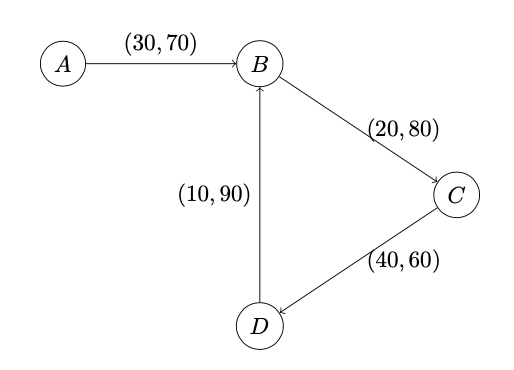
\includegraphics[width=0.5\textwidth]{figs/graph.png}
  \caption{Example of voting graph}
  \label{fig:q1_example}
\end{figure}

In this example, there will no be any Condorcet winner because the graph is not a directed acyclic graph, indeed there is a cycle between the candidates $B$, $C$ and $D$.
The RCVS is then needed to solve this problem. We simply need to compute the $A$ matrix respecting the graph represented in figure \ref{fig:q1_example} following the rule described in section \ref{sec:model}:

$$A = \begin{pmatrix}
  0 & -40 & 0 & 0\\
  40 & 0 & -60 & 80\\
  0 & 60 & 0 & -20\\
  0 & -80 & 20 & 0
\end{pmatrix}$$
\newpage
When lauching the \verb|q1_model.jl| file with this matrix as input, we obtain the following lottery for the RCVS :

\begin{table}[!h]
  \centering
  \begin{tabular}{|c|c|c|c|c|}
  \hline
  Candidate   & $A$   & $B$     & $C$   & $D$     \\ \hline
  Probability & $0.0$ & $0.125$ & $0.5$ & $0.375$ \\ \hline
  \end{tabular}
  \caption{Lottery probabilities for each candidate}
  \label{tab:q1_prob}
\end{table}

\subsection{Discussion of the dual variables and optimal dual basis}


\subsection{Solution of the linear in a linear system}


\subsection{\textit{Bonus} : Comparaison of the RCVS with an alternative voting system}